\section{Teoria da Ordenação}
\

O \textbf{problema da ordenação} é recorrente na ciência da computação, o motivo para isso é bem simples: Muitos problemas algorítmicos são mais fáceis de serem resolvidos quando os dados estão distribuídos de forma ordenada.

Nas próximas sub sessões serão apresentados alguns algoritmos de ordenação, inicialmente serão apresentados algoritmos ingênuos com complexidade polinomial, logo após, algoritmos de ordenação eficientes e por fim algoritmos com complexidade de tempo de execução linear. Para fins de simplificação, os algoritmos serão apresentados para ordenar vetores de números inteiros, no entanto, qualquer tipo de dado pode ser ordenado por um parâmetro. 

\subsection{Ordenação por bolha}
\

O algoritmo de ordenação por bolha ou ordenação por flutuação, ou ainda, do inglês \textit{bubble sort}, é um algoritmo de ordenação de complexidade de tempo de execução polinomial. O \textit{bubble sort} funciona (1) comparando um elemento com o imediatamente seguinte e (2) trocando-os caso os elementos adjacentes estejam desordenados. Esse algoritmo repete tais ações para sub vetores até que o vetor esteja ordenado.

\begin{figure}[h]
  \centering
  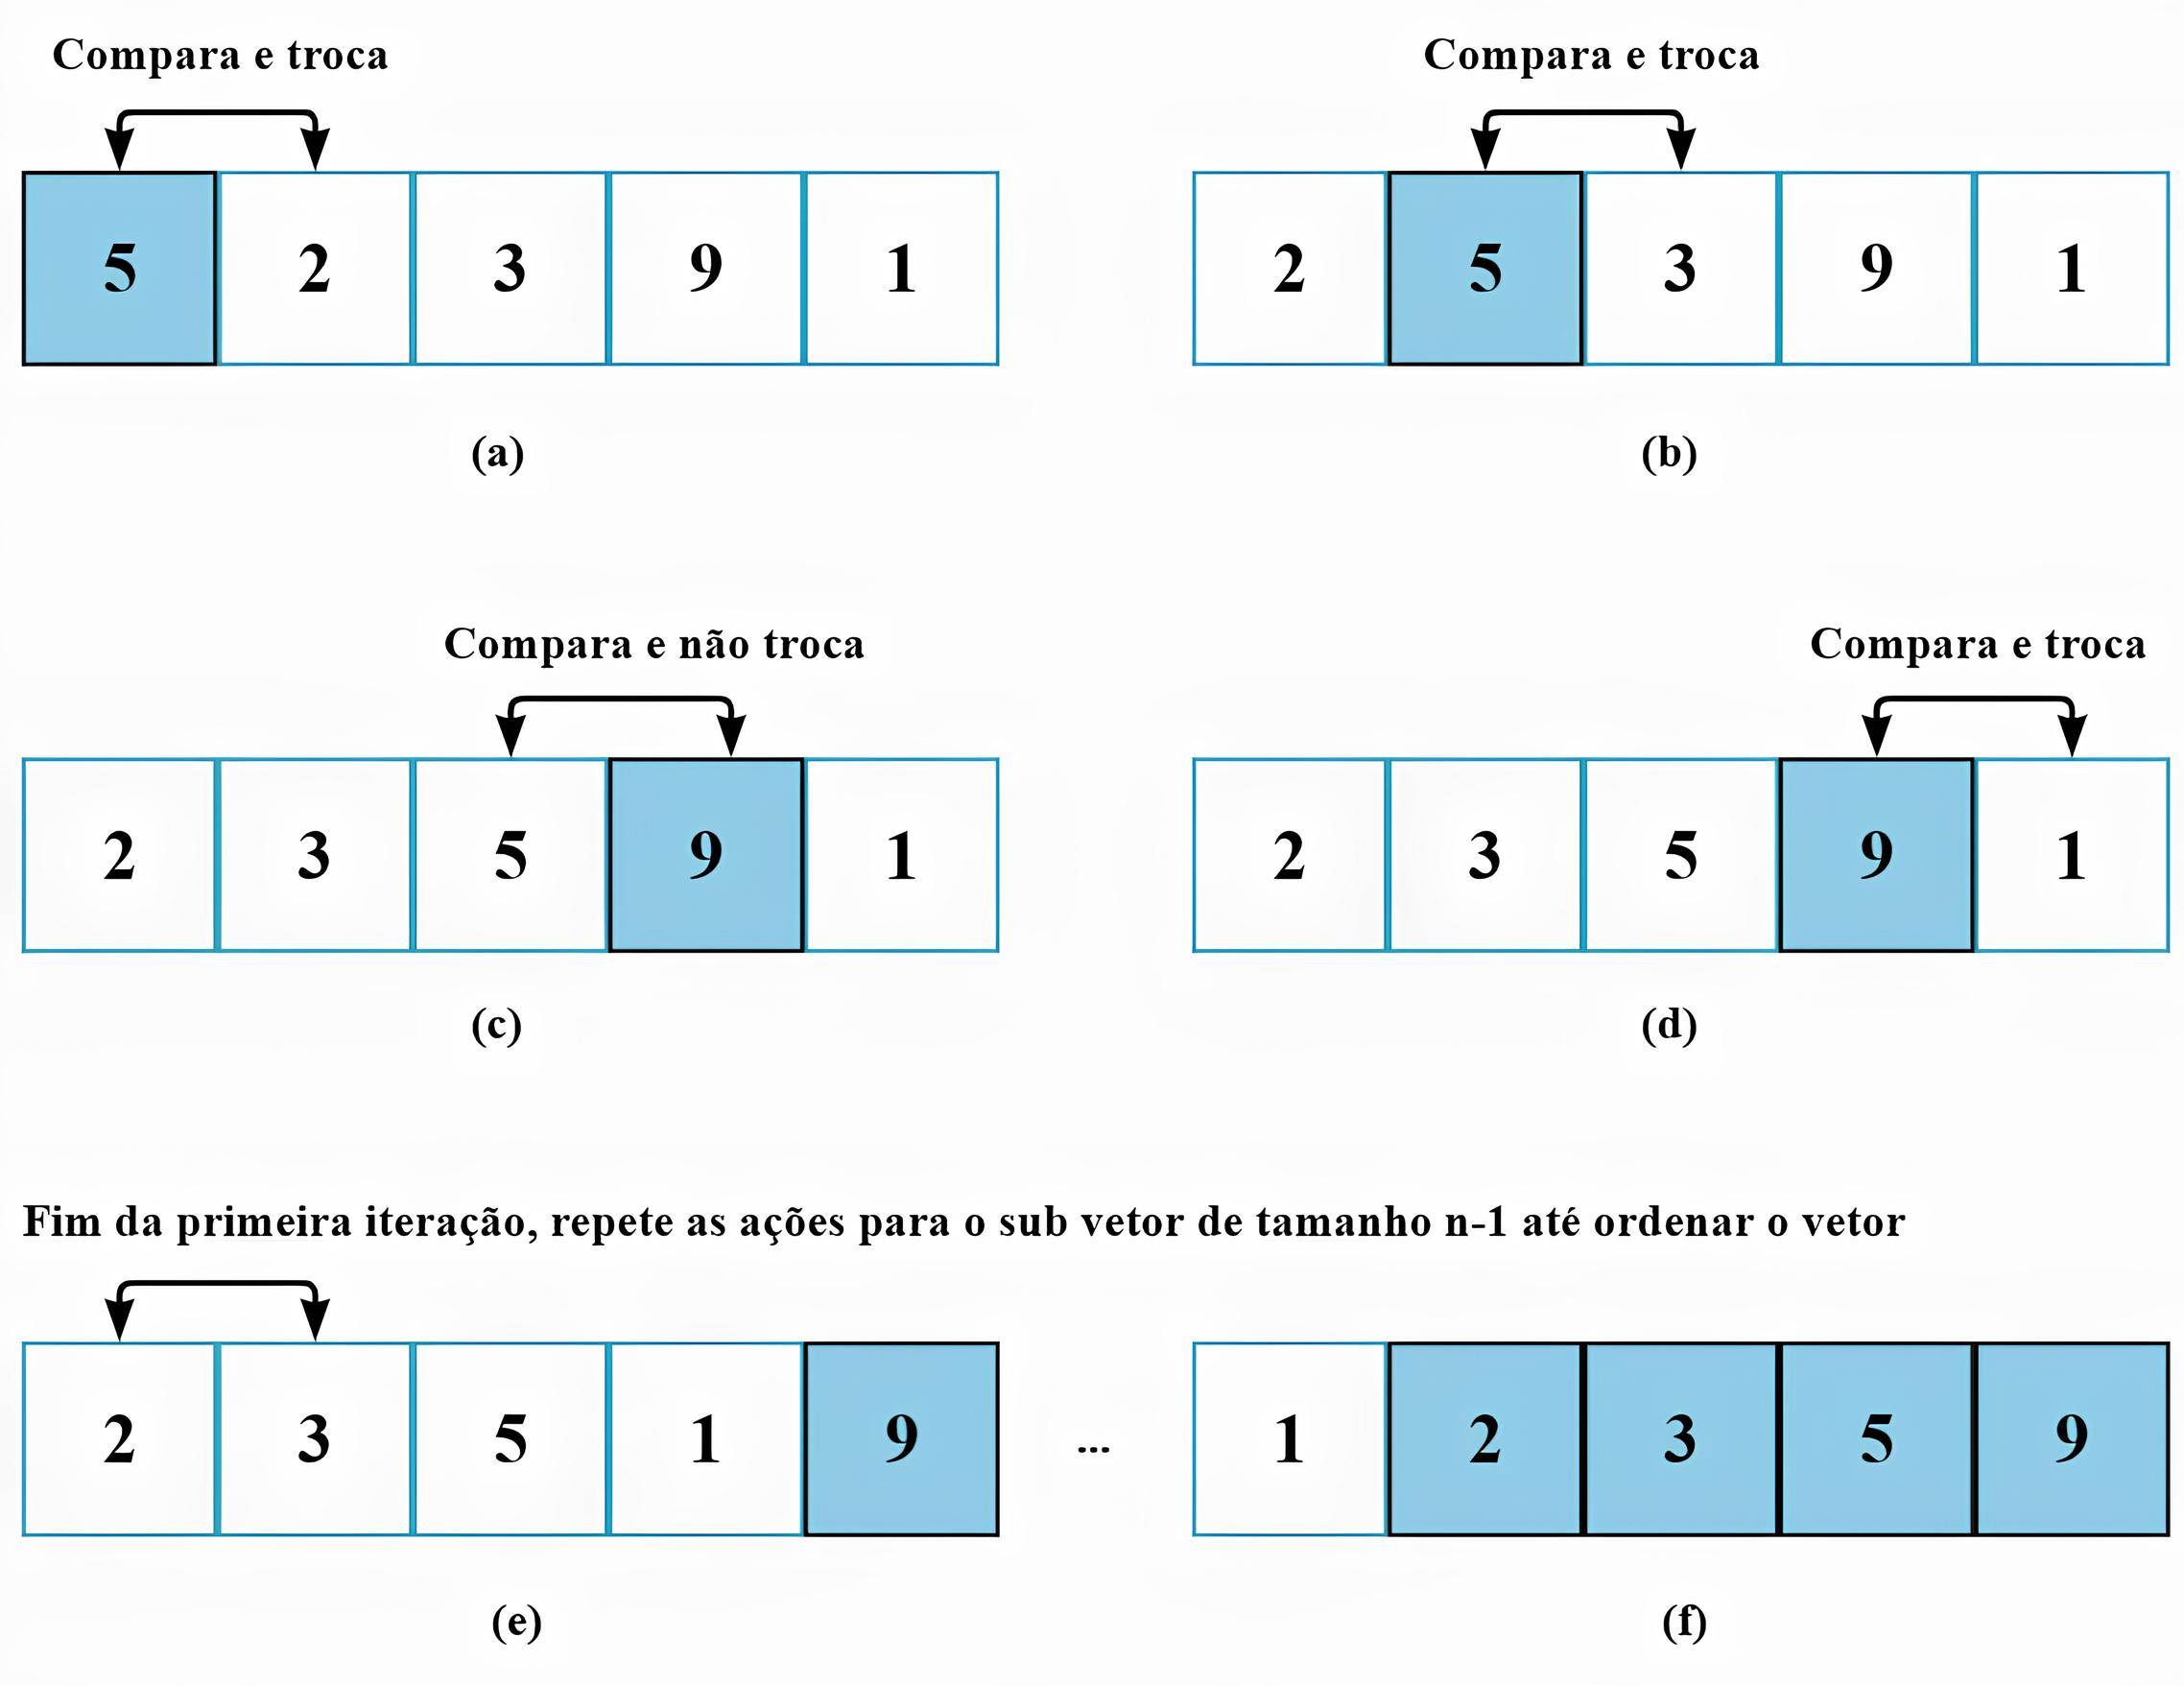
\includegraphics[width=.9\linewidth]{img/bubblesort.jpg}
  \caption{Ordenação por bolha atuando em um vetor cujo os elementos são números inteiros; Os elementos em azul são os maiores a cada iteração ou chamada do algoritmo e são postos no final do sub vetor e por fim ordenando o vetor por completo.}
  \label{bubblesort}
\end{figure}

É perceptível que as operações mais feitas no algoritmo em questão são as \textbf{comparações} e as \textbf{trocas}. O código em C a seguir descreve as instruções para algoritmo \texttt{bubble\_sort} que ordena um vetor de tamanho $n$ indexado de $0$ a $n-1$ cujo os elementos pertencem à $\mathbb{Z}$ . A função \texttt{swap} é responsável por trocar os elementos de posição, a flag \texttt{trocou} tem a funcionalidade de verificar se alguma troca foi efetuada, ela será útil pois, caso não seja realizadas trocas o vetor já está ordenado, no entanto as iterações ou chamadas podem ainda não ter chegado ao fim. Na melhor das hipóteses, caso o vetor já esteja ordenado basta uma iteração, pois a flag \texttt{trocou} dirá que nenhuma troca foi efetuada.

\begin{lstlisting}[language=C, frame=single]
    void bubble_sort(int *V, int n)
    {
        for(int i=0; i<n-1; i++)
        {
            int trocou = 0;
            for(int k=0; k<n-1-i; k++)
            {
                if(*(V+k)>*(V+k+1))
                {
                    swap(V+k, V+k+1);
                    trocou=1;
                }
            }
            if(trocou==0) break;
        }
    }
\end{lstlisting}

O código supracitado é uma versão iterativa do algoritmo que utiliza a flag de verificação de troca, também é possível implementar uma versão recursiva baseada em chamadas de sub vetores.

\begin{lstlisting}[language=C, frame=single]
    void bubble_sort_recursive(int *V, int n)
    {
        if(n<=1) return;
        int trocou = 0;
        for(int i=0; i<n-1; i++)
        {
            if(*(V+i)>*(V+i+1))
                {
                    swap(V+i, V+i+1);
                    trocou=1;
                }
        }
        if(trocou==0) return;

        bubble_sort_recursive(V, n-1);
    }
\end{lstlisting}

\subsubsection{Análise de complexidade}
\

A intuição por trás da análise de complexidade da ordenação por bolha é pensar que, no \textbf{pior caso}, todas as operações possíveis são realizadas, para que isso aconteça o vetor deve estar em ordem decrescente caso queiramos uma ordenação crescente.

Considere a versão não recursiva, é visível que 

(1) O primeiro laço de iteração \texttt{for} realiza seu procedimento interno $n-1$ vezes;

(2) O segundo laço tem um comportamento baseado no iterador \texttt{i}, onde seu procedimento interno é executado $n-1-i$ vezes, tem-se então

\[(n-1-0)+(n-1-1)+(n-1-2)+...+1 = \frac{(n-1)n}{2}\in O(n^2).\]

A análise acima é suficiente para demonstrar a cota superior da complexidade do tempo de execução. Se os índices do vetor forem pensados como elementos pertencentes à $\mathbb{N}$ então é possível escrever 

\[\sum_{i=1}^{n-1}\sum_{k=1}^{i-1}\kappa.\]

Onde $\kappa$ é uma constante que representa o custo da operação de troca. No \textbf{pior caso} essa constante é somada a cada iteração, já que a operação de troca é sempre feita.

\[\sum_{i=1}^{n-1}\sum_{k=1}^{i-1}\kappa = \sum_{i=1}^{n-1}\kappa(i-1) = \kappa[1+2+...+(n-2)+(n-1)]=\frac{\kappa(n-1)n}{2}.\]

Esse é o resultado obtido na análise intuitiva, agora basta provar que a progressão aritmética encontrada está em $O(n^2)$. Lembrando que $O(kg(n)) = kO(g(n)) = O(g(n))$, para demonstrar que $\frac{\kappa(n-1)n}{2} \in O(n^2)$, basta encontrar constantes $n_0$ , $k > 0$ tais que $\frac{(n-1)n}{2}\leq kn^2 \ \forall n\geq n_0$.

\[\frac{(n-1)n}{2}=\frac{n^2 - n}{2}\leq kn^2 \Rightarrow \Bigr(\frac{1}{2}-k\Bigr)n^2 - \frac{n}{2}\leq 0 \ \forall n\geq n_0.\]

Para satisfazer a inequação acima, basta escolher $k=\frac{1}{2}$ e $n_0=1$, substituindo

\[\Bigr(\frac{1}{2}-\frac{1}{2}\Bigr) - \frac{1}{2} \leq 0 \Rightarrow-\frac{1}{2} \leq 0; \ \therefore \frac{\kappa(n-1)n}{2}\in O(n^2).\]

{\raggedleft $\blacksquare $ \par}

A análise intuitiva do \textbf{melhor caso} é bem simples, quando a flag \texttt{trocou} não receber o valor $1$ significa que o vetor está ordenado. Se o vetor já estiver ordenado, apenas $n-1$ iterações no laço exterior são realizadas e ele termina a execução; $n-1 \in O(n)$, então a complexidade do tempo de execução do melhor caso é linear.

Considere no melhor caso que atribuir valor a flag tenha um custo constante $O(1)$ e que são realizadas $n-1$ comparações, mas nenhuma chamada de \texttt{swap}, portanto, nenhuma troca. Dessa forma, a flag será $0$ e a comparação final devolvera um retorno para o método, portanto a função complexidade é $f(n) = n-1+O(1)$, considerando que $\exists k > 0; \ n-1 \leq kn$, então $f(n) \in O(n)$. Sendo assim, a complexidade do tempo de execução no melhor caso para \texttt{bubble\_sort} está em $O(n)$.

{\raggedleft $\blacksquare $ \par}

Em penúltimo lugar, a análise de complexidade do \textbf{caso médio} para o tempo de execução do algoritmo de ordenação por bolha deve receber algumas considerações. Em primeiro lugar, considere que em metade das comparações são realizadas trocas, isso pode ser justificado se atribuirmos $0$ "uma comparação foi executada mas uma troca não foi executada" \ e $1$ "uma comparação foi executada e uma troca foi executada"; Assim sendo, o valor esperado $E[x]$ é igual a $\frac{1}{2}$. Obtem-se então

\[\sum_{i=1}^{n-1}\sum_{k=1}^{i-1}\frac{1}{2}\kappa = \frac{1}{2}\sum_{i=1}^{n-1}\kappa(i-1) =  \frac{\kappa (n-1)n}{4}\]

de $\frac{(n-1)n}{2} \in O(n^2)$ e $kO(f(n))=O(f(n))$ encontra-se o limite assintótico $\frac{\kappa(n-1)n}{4} \in O(n^2)$ que é a complexidade do tempo de execução do caso médio do algoritmo em questão.

{\raggedleft $\blacksquare $ \par}

Por fim, mas não menos importante, para avaliar o \textbf{complexidade de espaço} requerido para a ordenação por bolha não é considerado o espaço onde o vetor a ser ordenado está armazenado, pois o algoritmo em si não o armazena e nem cria cópias para manipular os elementos do vetor a ser ordenado.

No algoritmo para os iteradores \texttt{i} e \texttt{k}  e para a flag \texttt{trocou} considere um custo constante $1$, assim a função $s(n)$ complexidade de espaço é $s(n) = 3 \in O(1)$.

\subsubsection{Sumário ordenação por bolha}

\begin{table}[h]
\centering
\begin{tabular}{|c|c|c|c|c|}
\hline
\textbf{Algoritmo} & \textbf{Pior caso} & \textbf{Caso médio} & \textbf{Melhor caso} & \textbf{Estabilidade} \\ \hline
Ordenação por bolha       & \(O(n^2)\)         & \(O(n^2)\)             & \(O(n)\)           & Estável                \\ \hline
\end{tabular}
\caption{Complexidade e estabilidade do Algoritmo de ordenação por bolha.}
\label{Sumario bubble sort}
\end{table}
